\chapter{Eredmények, tapasztalatok, továbbfejlesztési lehetőségek}
Az Orange Crush 20L gitárerősítő áramkörét modelleztem, és VST3 plugint írtam belőle a JUCE fejlesztői környezetben. Az erősítő áramkör minden része elkészült, kivéve a tone stack része. Az egyes megvalósult részeket összerakva egy működő plugin a végeredmény.

A plugin tesztelése többféle bemenő jelre is megtörtént, az LTSpice szimulációkkal hasonlítottam össze. A tone stack rész megvalósítása nem történt meg, így a szimulációkban az áramköri részét rövidre zártam. 
\begin{figure}[H]
    \centering
    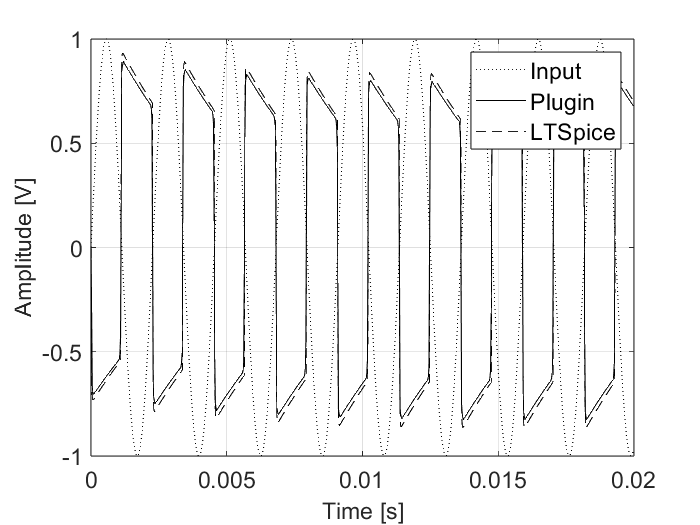
\includegraphics[scale=0.5]{figures/final.png}
    \caption{Az elkészült plugin tesztelése és összehasonlítása LTSpice szimulációval. A GAIN és az OVERDRIVE paraméter maximumon van ennél az összehasonlításnál, a bemenő jel egy $440Hz$ frekvenciájú szinusz jel.}
\end{figure}
\section{Tapasztalatok}
Az elkészítés során megszerzett tapasztalatok:
\begin{itemize}
    \item A torzító részben, amit K-módszerrel valósítottam meg van egy OVERDRIVE paraméter, aminek a változása esetén mindig újra kell számolnom a (\ref{G}), (\ref{H}), (\ref{J}), (\ref{K}) segédváltozókat, és az eredeti nemlineáris egyenletemet újra lineárisan transzformálva újra kell generálni 
    a táblázatot a K-módszer futtatásához.
    \item A K-módszer megvalósításához először a $juce::dsp::Matrix<type>$ előre megírt osztályt használtam a mátrixműveletek elvégzéséhez. Viszont ennek az osztálynak a használatával a plugin nem működött megfelelően, folyamatosan recsegő hangok voltak hallhatóak a kimenet mellett. A saját mátrix osztályom megírása és használata után ez a probléma megoldódott.
    \item A tone stack résznél a sok paraméter miatt nagyon körülményes az átvitel felírása.
    \item A modell a valóságot modellezi, így a valóság feszültségszintjei szerint kell a bemenő és a kimenő jelet értelmezni. Ezt úgy oldottam meg, hogy megnéztem egy átlagos gitárjel maximum értéke milyen szám körüli, és így a bemenetre ezt felszoroztam annyival, hogy egy valóságos gitárjel feszültségértékeinek feleljenek meg az értékek (körülbelül $0.5-1.5V$). A kimenetre rakott feszültséglevágás miatt a kimenetet pedig csak egyszerűen leosztottam.
    \item A K-módszer táblázatába alapból $1000$ pontpárt generáltattam le legelőször, és ez a mennyiség egyáltalán nem okozott problémát a futás közben. A táblázat elemei között elég volt lineárisan interpolálni, nem volt szükséges magasabb fokú interpolációra. 
\end{itemize}
\section{Továbbfejlesztése lehetőségek}
\begin{itemize}
    \item A tone stack megvalósítása.
    \item A torzítások miatt az eredeti jel alapharmonikusának felharmonikusai meg fognak jelenni a kimeneten. Ez a mintavételi tétel megszegését okozhatja, és átlapolódás keletkezhet. Mindenképpen célszerű lenne a pluginhoz egy mintavételi frekvencia konvertáló osztályt megírni, amivel először a jelet a torzító részek előtt interpolálom, majd a torzító részek után pedig szűröm és decimálom. Ezzel a mintavételi frekvencia felét átlépő frekvenciák ki lennének szűrve, és nem okozhatnának átlapolódást.
    \item A paraméterek ne ugrásszerűen, hanem lineárisan változva érjék el az új értéket.
    \item A torzító részben a műveleti erősítő egyes paraméterállásoknál levág, ezt is célszerű lenne megvalósítani az eredeti hangzás érdekében.
\end{itemize}